% !TeX program = pdflatex
\documentclass[border=6pt]{standalone}
\usepackage{amsmath}
\usepackage{tikz}
\usetikzlibrary{arrows.meta, positioning, calc}

\definecolor{MediumRed}{rgb}{0.925, 0.345, 0.345}
\definecolor{MediumGreen}{rgb}{0.37, 0.7, 0.66}
\definecolor{MediumBlue}{rgb}{0.015, 0.315, 0.45}
\definecolor{DarkBlue}{rgb}{0.05, 0.15, 0.35}

\begin{document}
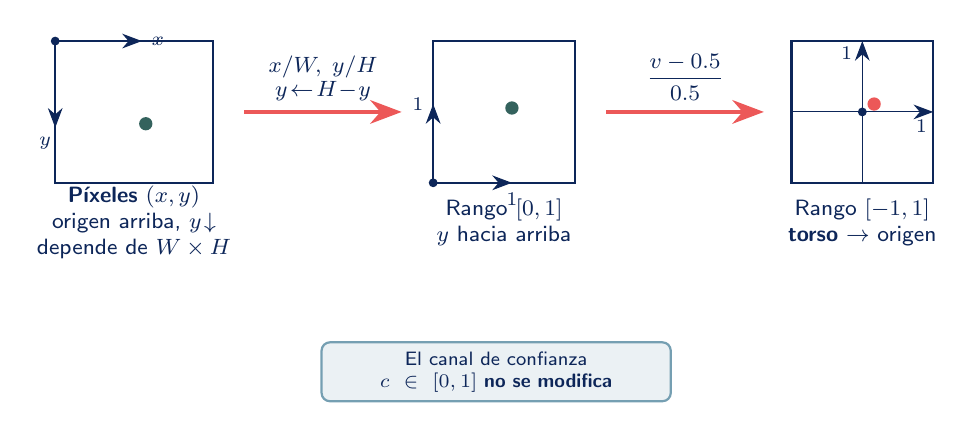
\begin{tikzpicture}[
    font=\sffamily,
    flow/.style={-{Stealth[length=4mm]}, line width=1.4pt, MediumRed},
    lbl/.style={font=\sffamily\footnotesize, text=DarkBlue},
]

% ============ ETAPA 1: pixeles absolutos ============
\begin{scope}[shift={(0,0)}]
    \draw[DarkBlue, thick] (0,0) rectangle (2,1.8);
    % origen arriba-izquierda, y hacia abajo
    \fill[DarkBlue] (0,1.8) circle (1.6pt);
    \draw[-{Stealth[length=2.5mm]}, DarkBlue] (0,1.8)--(1.1,1.8) node[right, font=\scriptsize] {$x$};
    \draw[-{Stealth[length=2.5mm]}, DarkBlue] (0,1.8)--(0,0.7) node[below left, font=\scriptsize, xshift=2pt] {$y$};
    \fill[MediumGreen!55!black] (1.15,0.75) circle (2.4pt);
    \node[lbl, align=center] at (1,-0.5) {\textbf{Píxeles} $(x,y)$\\ origen arriba, $y\!\downarrow$\\ depende de $W\times H$};
\end{scope}

\draw[flow] (2.4,0.9) -- node[above, lbl, align=center] {$x/W,\;y/H$\\[-1pt]$y\!\leftarrow\! H\!-\!y$} (4.4,0.9);

% ============ ETAPA 2: [0,1] eje invertido ============
\begin{scope}[shift={(4.8,0)}]
    \draw[DarkBlue, thick] (0,0) rectangle (1.8,1.8);
    \fill[DarkBlue] (0,0) circle (1.6pt);
    \draw[-{Stealth[length=2.5mm]}, DarkBlue] (0,0)--(1.0,0) node[below, font=\scriptsize] {$1$};
    \draw[-{Stealth[length=2.5mm]}, DarkBlue] (0,0)--(0,1.0) node[left, font=\scriptsize] {$1$};
    \fill[MediumGreen!55!black] (1.0,0.95) circle (2.4pt);
    \node[lbl, align=center] at (0.9,-0.5) {Rango $[0,1]$\\ $y$ hacia arriba};
\end{scope}

\draw[flow] (7.0,0.9) -- node[above, lbl, align=center] {$\dfrac{v-0.5}{0.5}$} (9,0.9);

% ============ ETAPA 3: [-1,1] centrado ============
\begin{scope}[shift={(10.25,0.9)}]
    \draw[DarkBlue, thick] (-0.9,-0.9) rectangle (0.9,0.9);
    \draw[-{Stealth[length=2.5mm]}, DarkBlue] (-0.9,0)--(0.9,0);
    \draw[-{Stealth[length=2.5mm]}, DarkBlue] (0,-0.9)--(0,0.9);
    \node[font=\scriptsize, text=DarkBlue] at (0.75,-0.18) {$1$};
    \node[font=\scriptsize, text=DarkBlue] at (-0.2,0.75) {$1$};
    \fill[DarkBlue] (0,0) circle (1.6pt);
    \fill[MediumRed] (0.15,0.1) circle (2.4pt);
    \node[lbl, align=center] at (0,-1.4) {Rango $[-1,1]$\\ \textbf{torso} $\rightarrow$ origen};
\end{scope}

% nota canal de confianza
\node[draw=MediumBlue!55, thick, rounded corners=3pt, fill=MediumBlue!8, text=DarkBlue,
      font=\sffamily\scriptsize, align=center, text width=4.2cm] at (5.6,-2.4)
    {El canal de confianza $c\in[0,1]$ \textbf{no se modifica}};

\end{tikzpicture}
\end{document}
